\documentclass[a4paper, 12pt]{article}

\usepackage{graphicx}
\usepackage[font=small, labelfont=bf, labelsep=colon]{caption}
\usepackage{amsmath, amssymb}
\usepackage{float}
\usepackage{xcolor}
\usepackage{hyperref}

\linespread{1.1}
\hypersetup{
colorlinks = true,
linkcolor = {blue!80!black}
}
\graphicspath{{../../Pictures/Simulation_histograms/}}
\renewcommand{\floatpagefraction}{0.99}

\title{Histograms of simulated Gas consumption}

\author{}
\date{}

\addtolength{\textwidth}{4cm}
\addtolength{\hoffset}{-2cm}
\setlength{\topmargin}{-2cm}
\addtolength{\textheight}{5cm}

\newcommand{\spc}{1ex}

\begin{document}
\maketitle
 
The histograms below concern simulated gas consumption of the energy model run by Aaron and Mohammad in Newcastle (the model simulates the energy consumption in Mohammad's house). Both batches consist of 1,000 simulations: in batch 1 six input variables are varied; in batch 2, two further inputs are varied.
Data about the monthly consumption is available and represented in each plot by a blue vertical line.


\begin{figure}
\centering
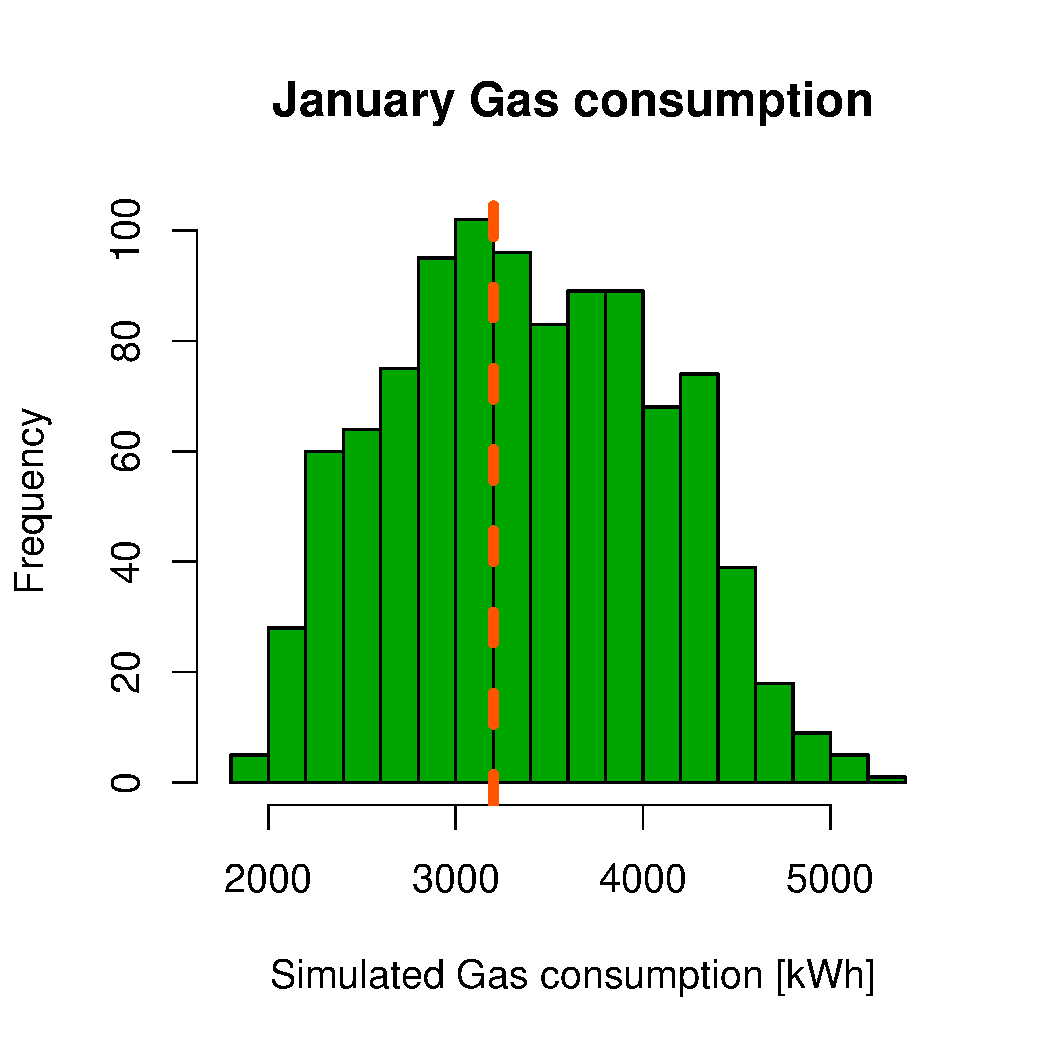
\includegraphics[width=0.49\textwidth]{January_Gas.pdf}
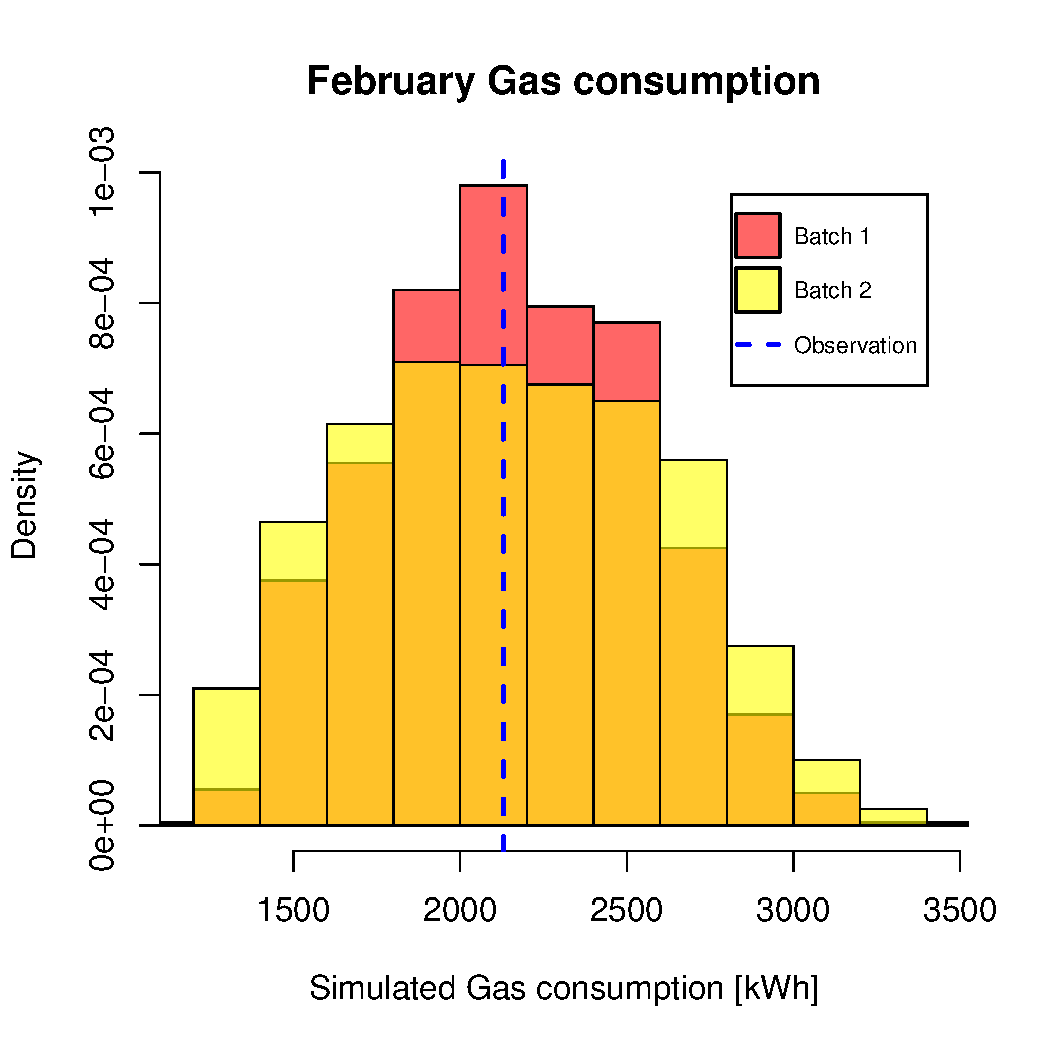
\includegraphics[width=0.49\textwidth]{February_Gas.pdf}
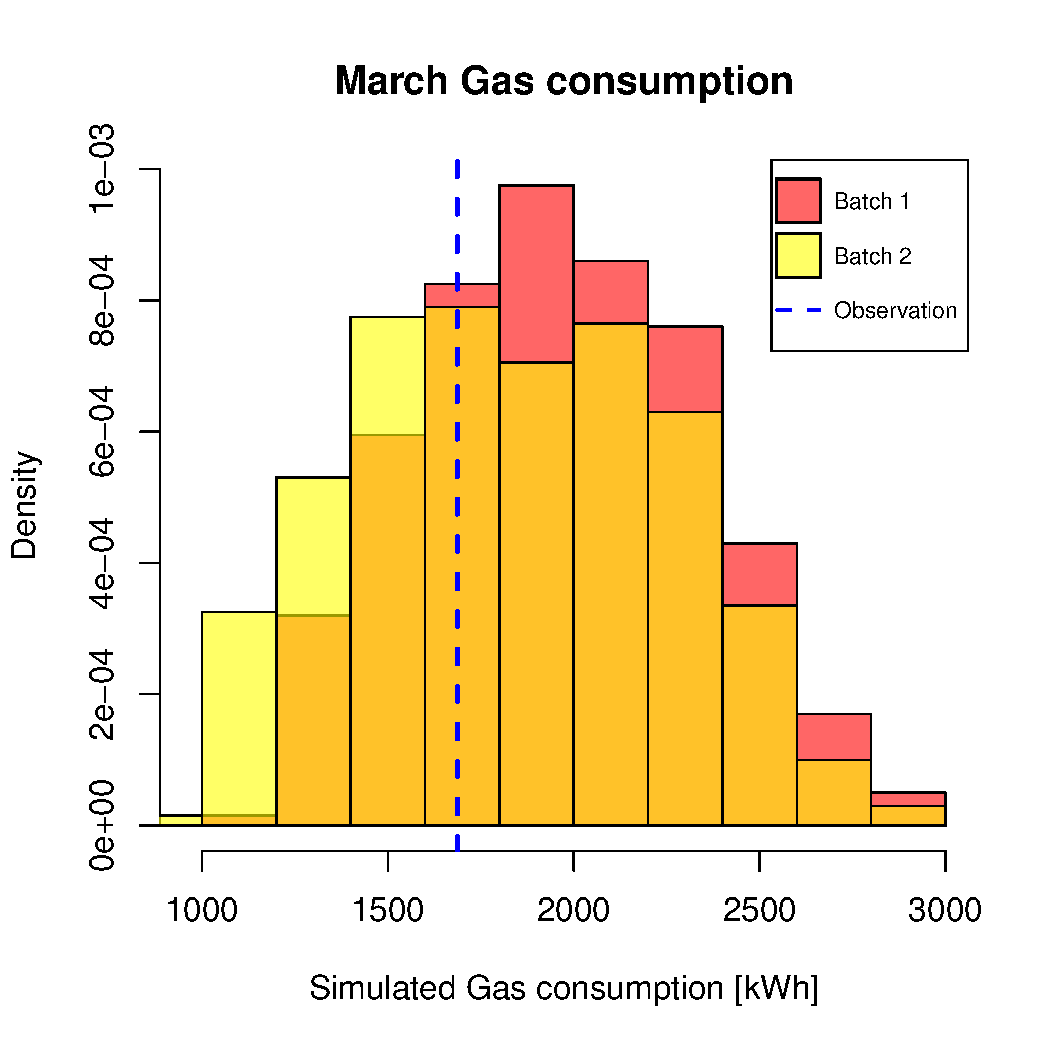
\includegraphics[width=0.49\textwidth]{March_Gas.pdf}
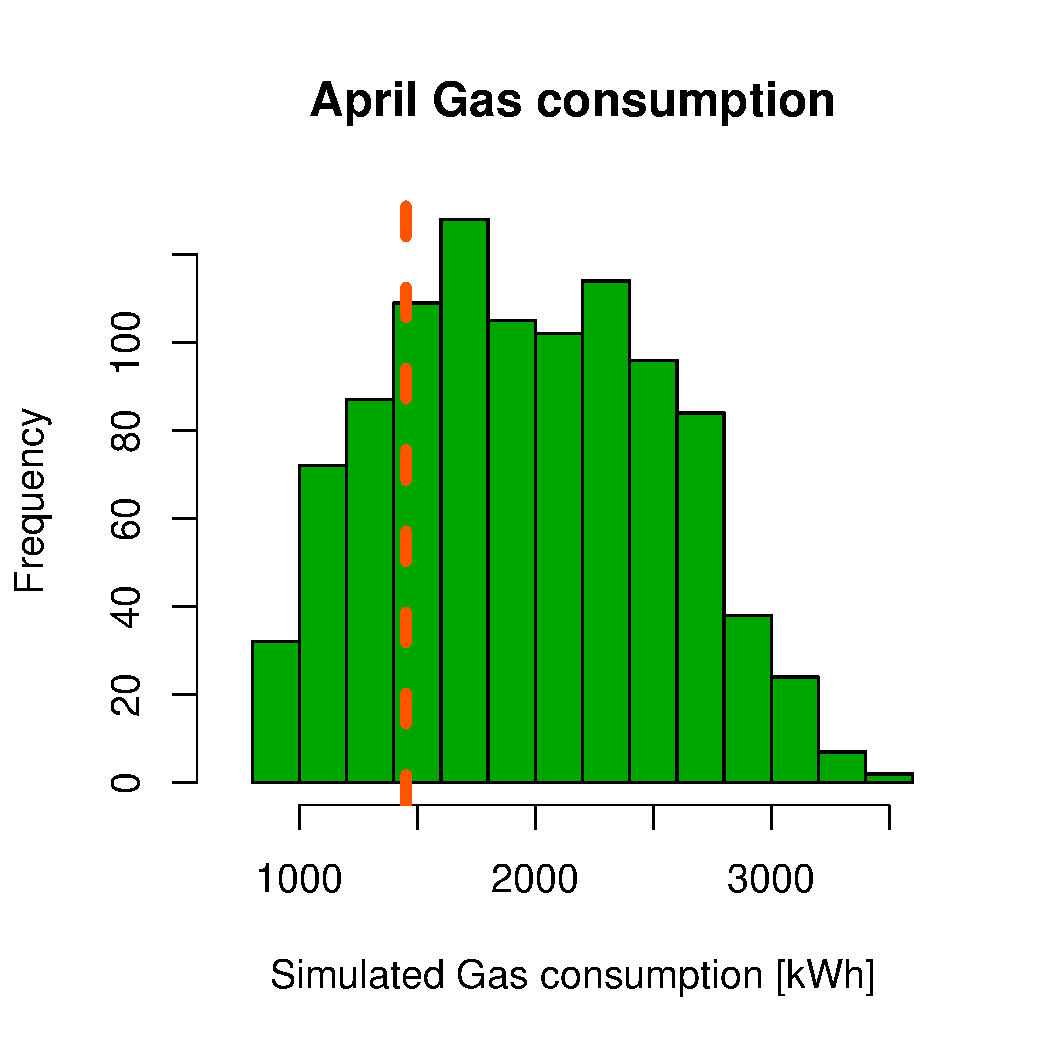
\includegraphics[width=0.49\textwidth]{April_Gas.pdf}
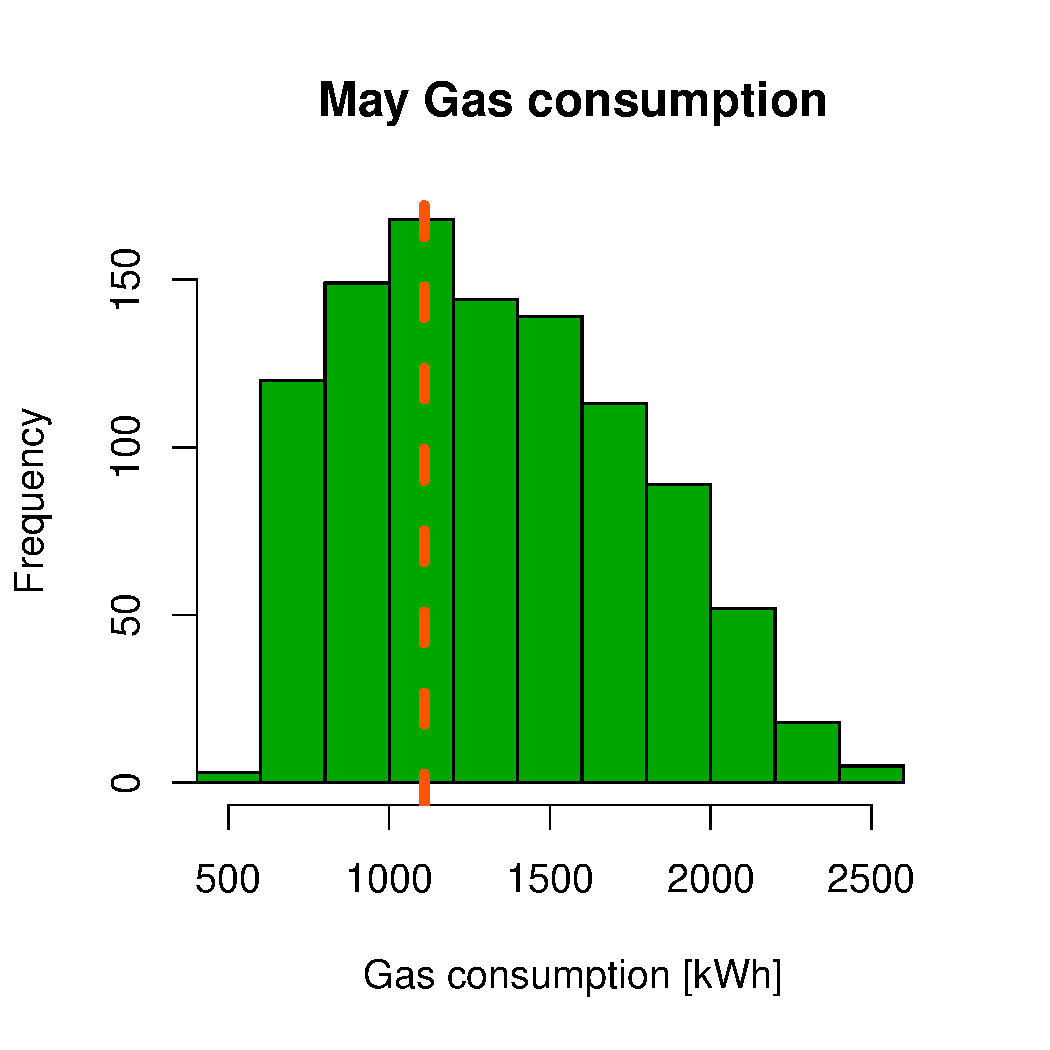
\includegraphics[width=0.49\textwidth]{May_Gas.pdf}
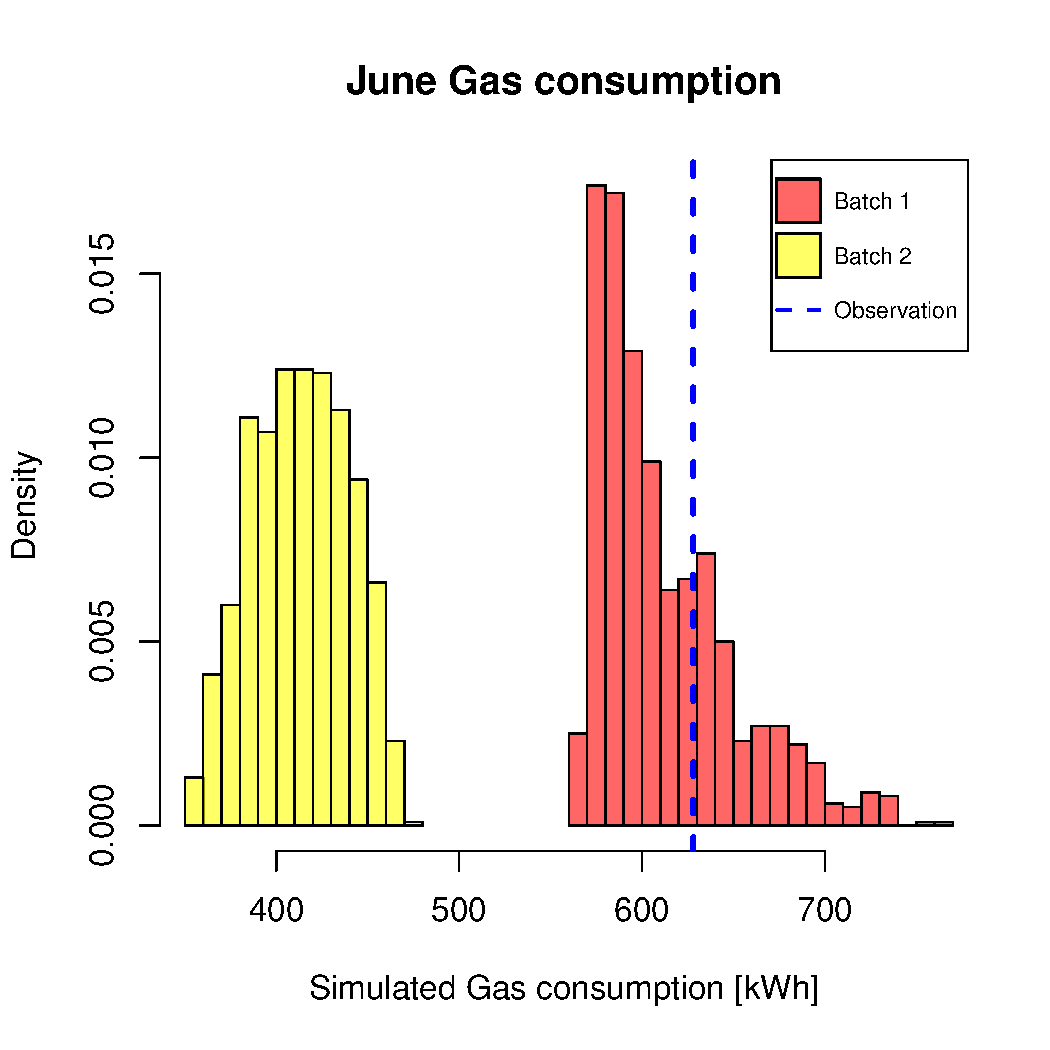
\includegraphics[width=0.49\textwidth]{June_Gas.pdf}
\end{figure}


\begin{figure}
\centering
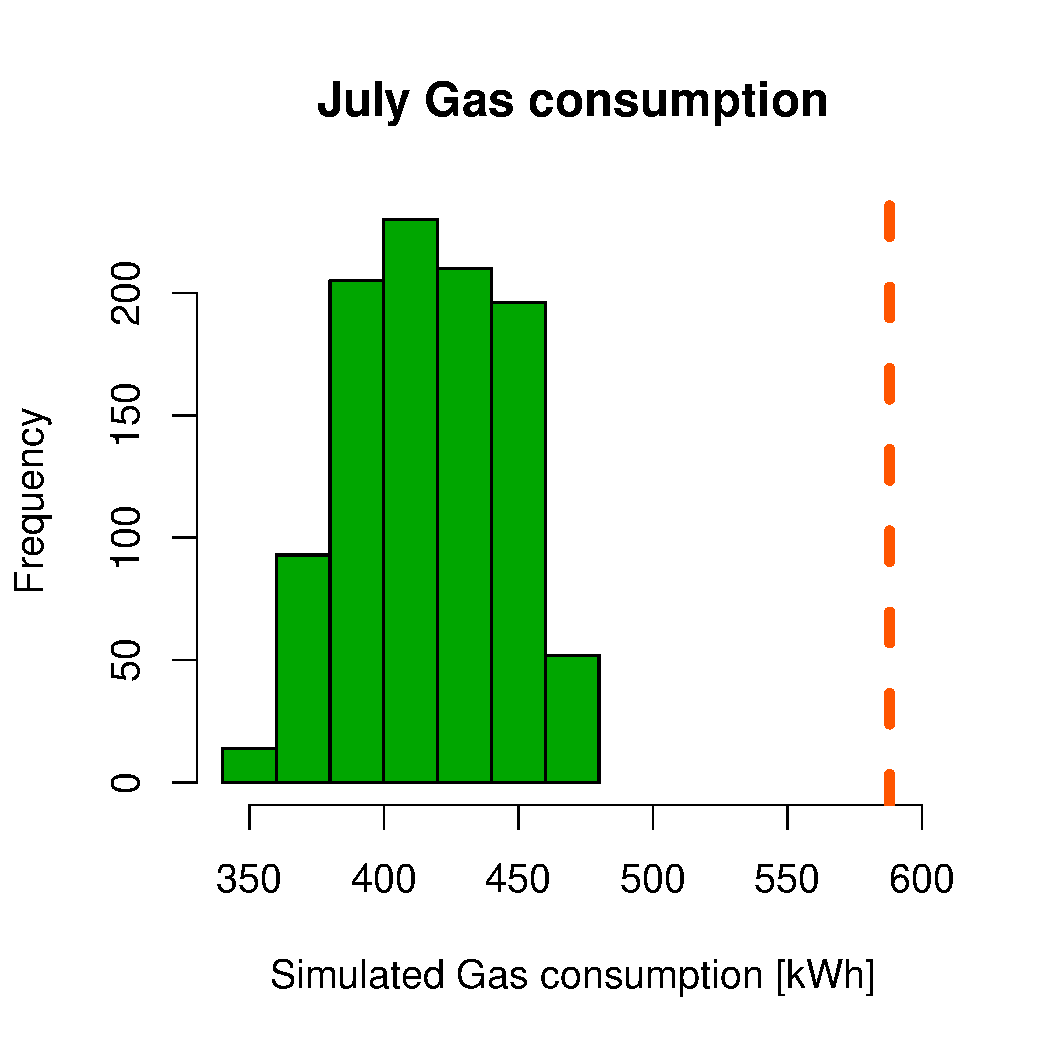
\includegraphics[width=0.49\textwidth]{July_Gas.pdf}
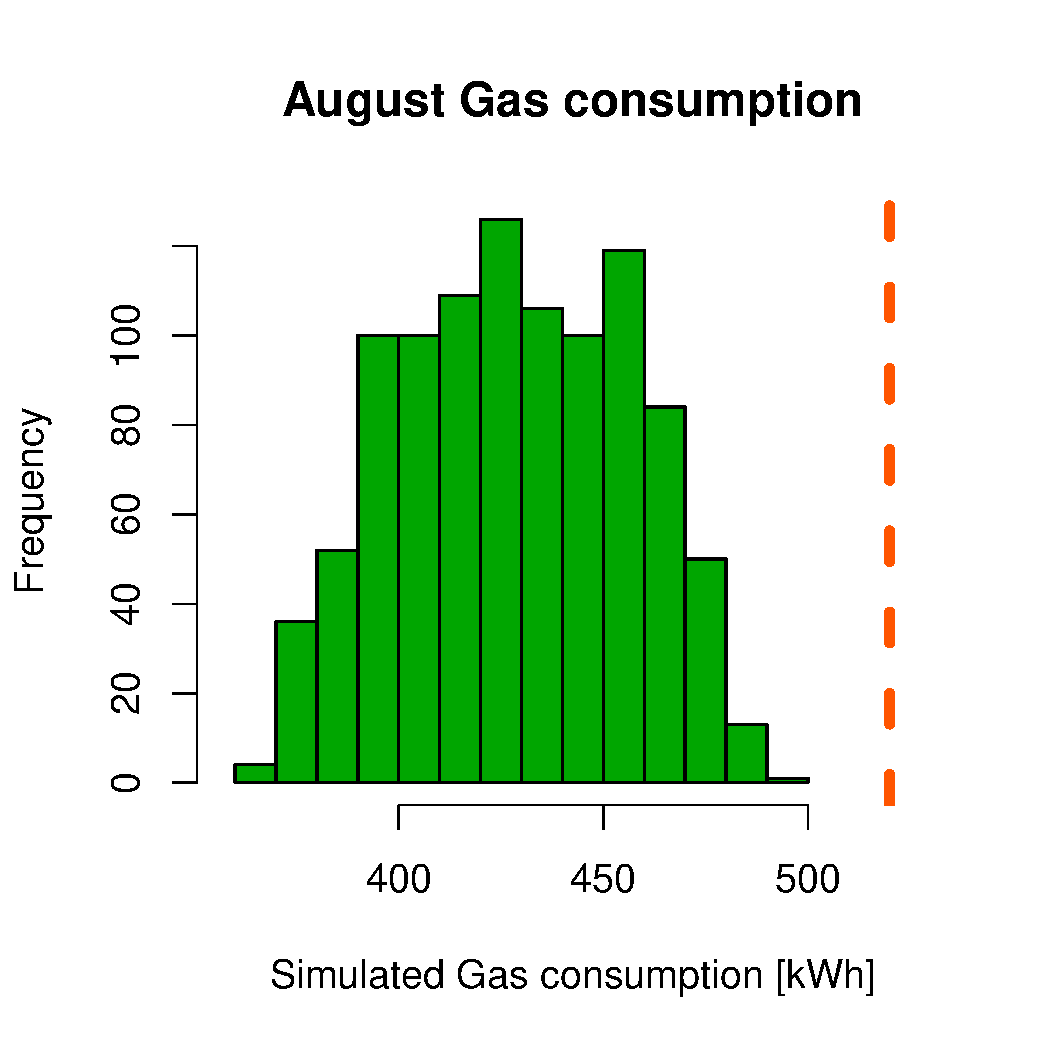
\includegraphics[width=0.49\textwidth]{August_Gas.pdf}
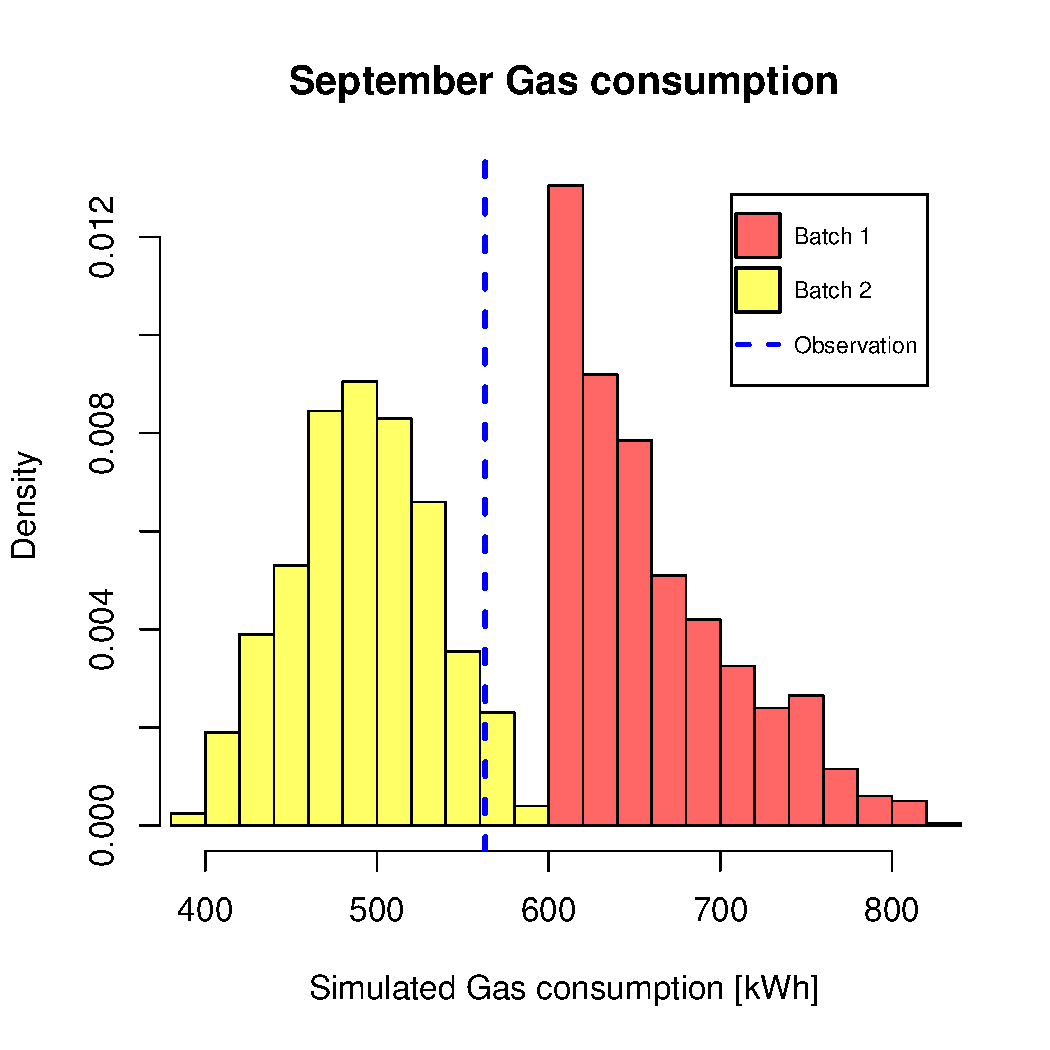
\includegraphics[width=0.49\textwidth]{September_Gas.pdf}
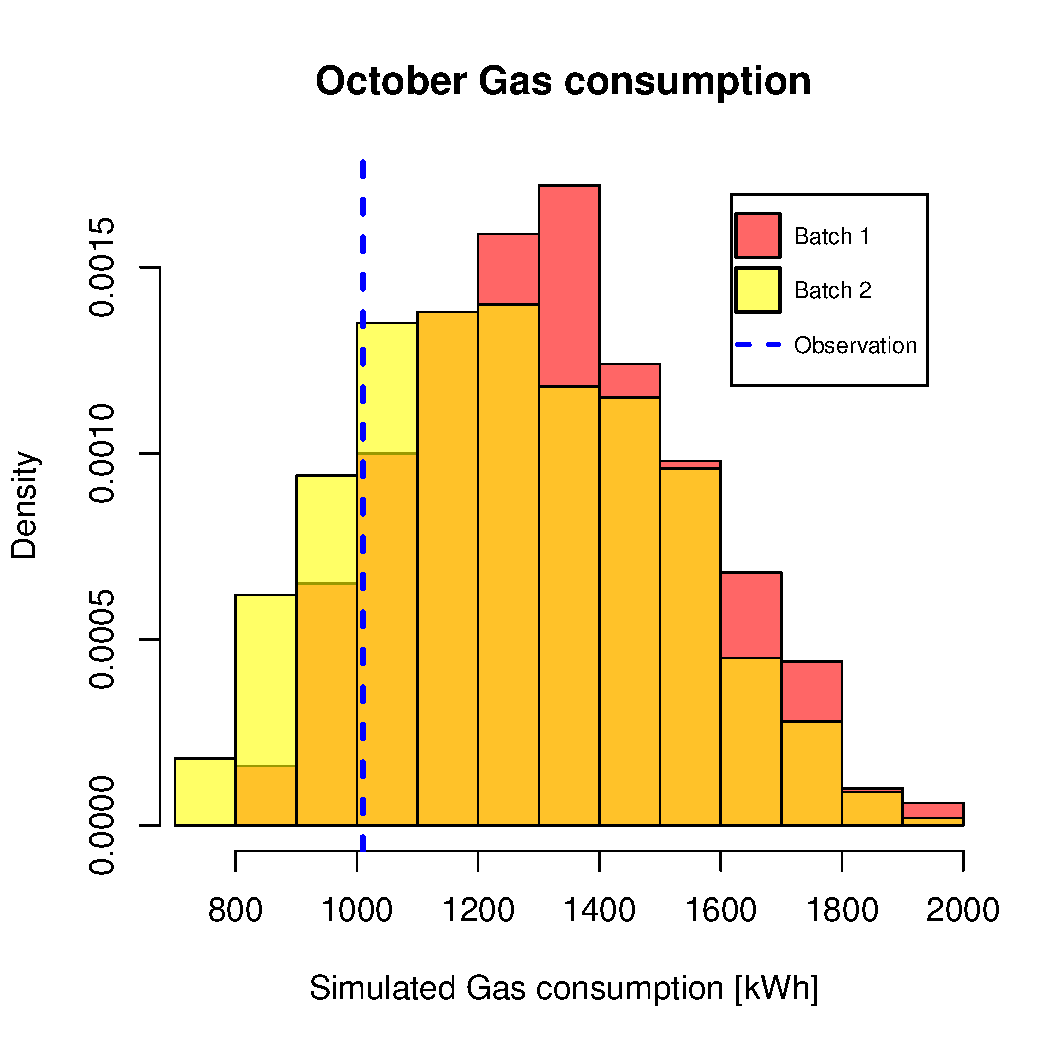
\includegraphics[width=0.49\textwidth]{October_Gas.pdf}
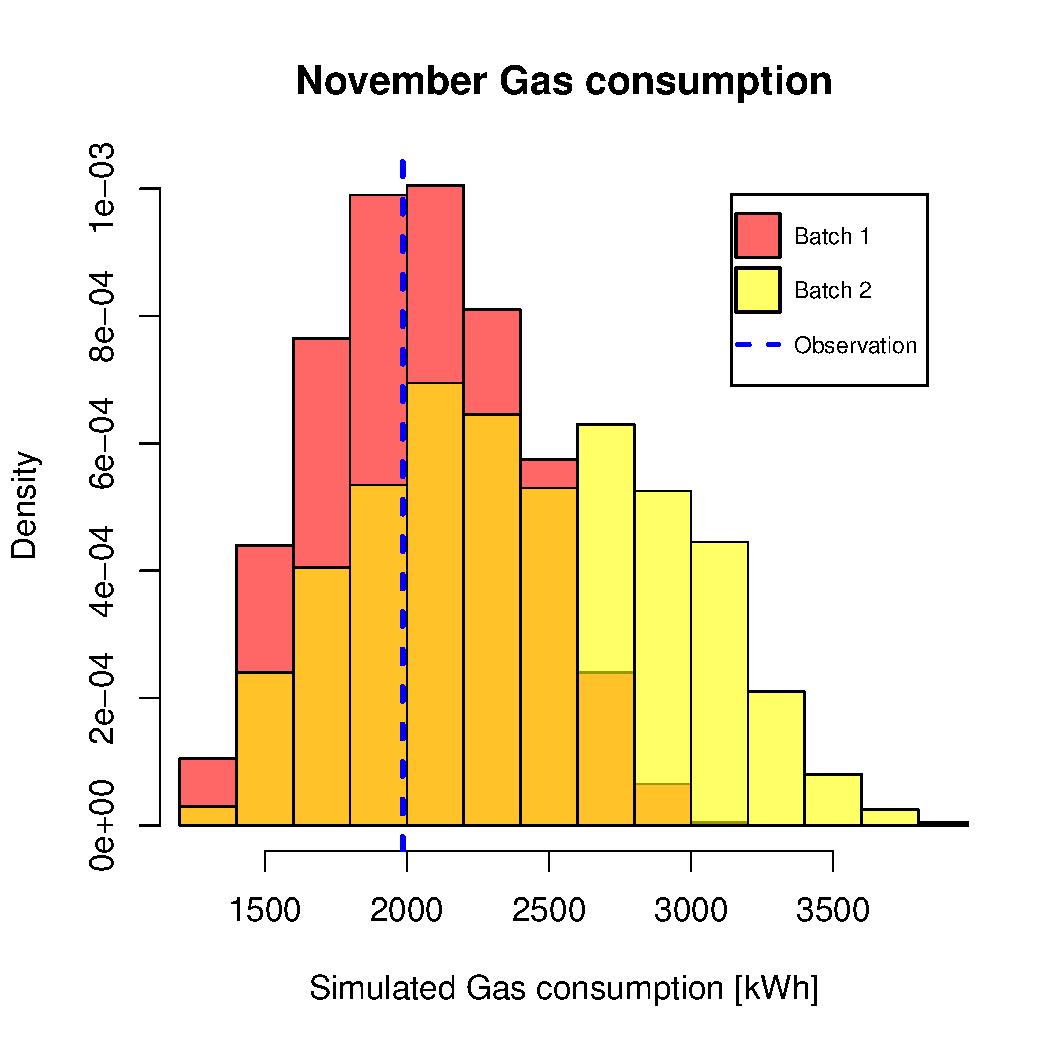
\includegraphics[width=0.49\textwidth]{November_Gas.pdf}
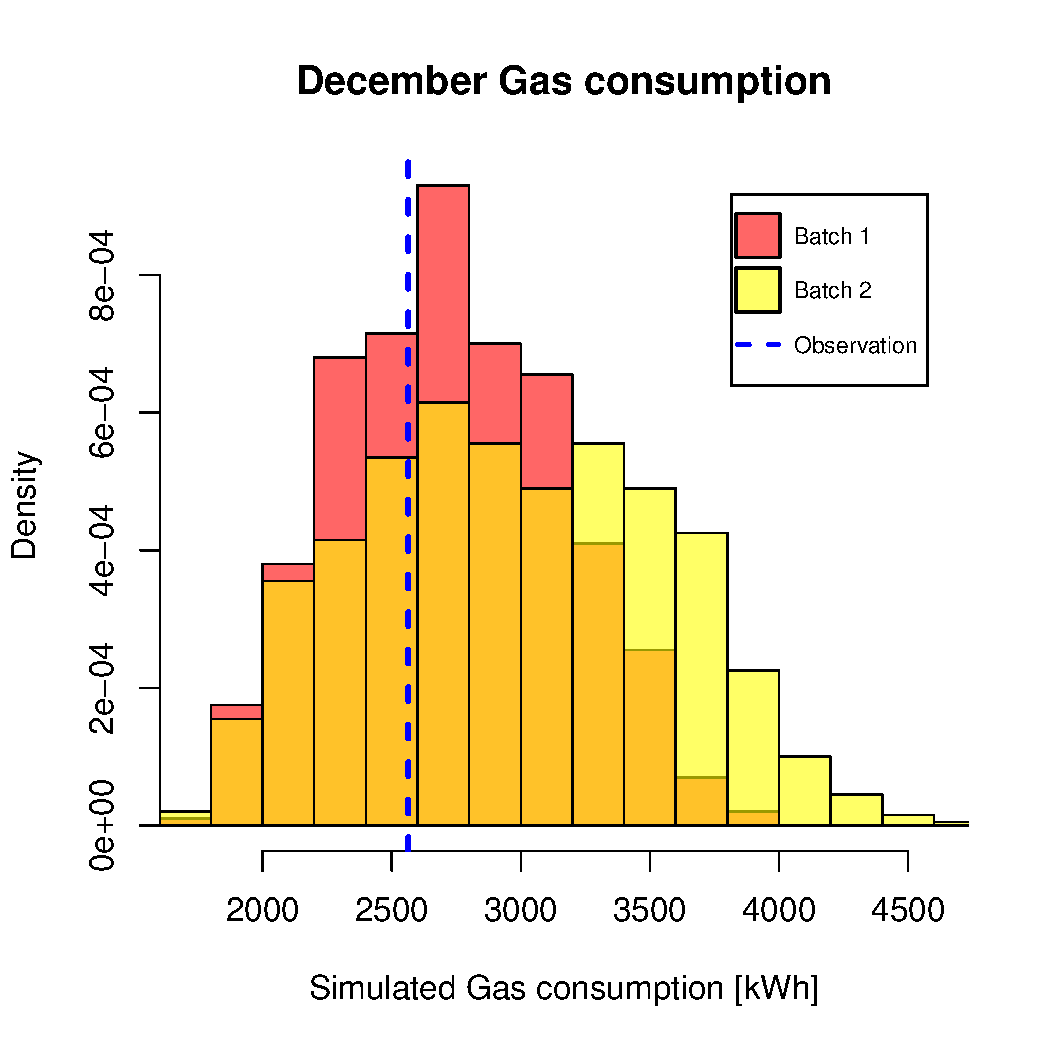
\includegraphics[width=0.49\textwidth]{December_Gas.pdf}
\end{figure}


\end{document}
